\section{Methodology}
\label{sec:methodology}
\subsection{Overview}
We predict whether the next JISDOR fixing is higher or lower than today's, using the market history and the news published up to the decision date. The study has four steps. First, we align each fixing with the articles of its decision day and label it UP or DOWN. Second, we turn the articles into one vector per day with a frozen encoder, so no language model is trained. Third, three levels of models answer the three questions in Section~I. Level~1 adds news to market features and checks whether the content matters beyond the article count. Level~2 swaps the text representation. Level~3 adds learned pooling, cross-attention, and a gate on the best representation. Fourth, we score every model on a chronological test period and then inspect why the scores look as they do.

\subsection{Dataset}
The market series contains the 1{,}202 JISDOR fixings from 2021-09-01 to 2026-09-01. The news corpus has 16{,}723 articles collected for geopolitical topics, 412 from the original collection and 16{,}311 from CNBC. Not every article reaches a decision row, since the earliest ones precede the first fixing, and the corpus metadata marks geopolitical relevance as audit-only, so some titles are not obviously geopolitical. Each article is represented by its headline and the first 180 cleaned body words. An article enters the first fixing strictly later than its source date, because only dates, not publication times, are available. We cannot verify historical publication times or article versions.

The label is the sign of the next fixing against the current one. $y=1$ (UP) means USD/IDR rises, so the rupiah depreciates. Exact ties are unlabeled. The 14 market inputs are lagged returns, 5- and 20-day volatility, moving-average ratios, momentum, RSI, the gap since the last fixing, and the weekday. All use data up to the decision date. Two availability inputs record the log article count and whether any article is present. Every decision has at least two articles, so the presence input is always 1.

The final 20\% of the calendar is the test period: 235 decisions from 2025-08-29 to 2026-08-31. The remaining 930 decisions form three expanding validation folds (train 453, 612, 772; validation 158, 159, 158). Rows at each boundary are purged so that no training label ends after the next period starts. Scalers, the TF-IDF vocabulary, and SVD are fitted on training rows only. Table~\ref{tab:splits} lists the periods. The share of UP days moves from 56.6\% in training to 50.0\% in validation and 58.3\% in test. Fig.~\ref{fig:eda} shows the series and the news coverage. Articles per decision day are right-skewed, with a median of 12, a 90th percentile of 23, and a maximum of 139.

% Copied from data/final/{train,val,test}.csv via eda-visualization/make_eda_figures.py.
\begin{table}[t]
    \caption{Decision periods. UP is the share of rising USD/IDR days.}
    \label{tab:splits}
    \centering
    \scriptsize
    \setlength{\tabcolsep}{3pt}
    \begin{tabular}{lcccc}
        \toprule
        Split & Period & Decisions & UP (\%) & Articles/day \\
        \midrule
        Train & 2021-09-29 to 2024-12-12 & 772 & 56.6 & 14.1 \\
        Validation & 2024-12-16 to 2025-08-26 & 158 & 50.0 & 12.3 \\
        Test & 2025-08-29 to 2026-08-31 & 235 & 58.3 & 15.0 \\
        \bottomrule
    \end{tabular}
\end{table}

% Generated by eda-visualization/make_eda_figures.py from data/final and data/processed.
\begin{figure*}[t]
    \centering
    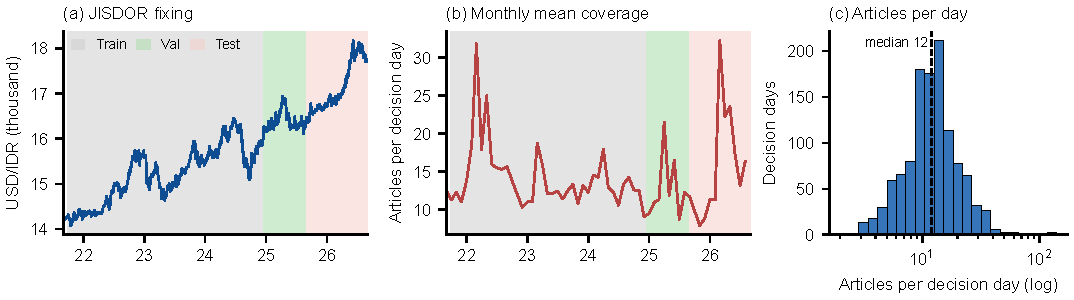
\includegraphics[width=\textwidth]{eda_overview}
    \caption{Data overview: (a) USD/IDR fixings by split, (b) monthly mean articles per decision day, (c) articles per decision day (dashed line: median).}
    \label{fig:eda}
\end{figure*}


\subsection{Evaluation}
Each model is refit on all 930 development decisions and scored on the test period with a fixed threshold of 0.5. MCC is the primary metric. With TP, TN, FP, and FN as the counts of true and false positives and negatives over $N$ test decisions, and $p_i$ the predicted probability of UP,
\begin{align}
\mathrm{Acc} &= \frac{TP+TN}{N},\\
\mathrm{MCC} &= \frac{TP\cdot TN - FP\cdot FN}{D},\\
\mathrm{LL} &= -\frac{1}{N}\sum_{i=1}^{N}\big[y_i\log p_i + (1-y_i)\log(1-p_i)\big].
\end{align}
where $D$ is the square root of the product of the four row and column totals. ROC-AUC is the probability that a random UP day receives a higher $p_i$ than a random DOWN day, with ties counting one half. MCC is defined as 0 for any constant prediction. Log loss clips probabilities at $10^{-15}$. How to read the scores: MCC runs from $-1$ to 1, where 0 means no better than chance and negative values mean predictions that tend to be wrong. Accuracy must be compared with the share of UP days, 0.583 in the test period, because a rule that always says UP already reaches it. AUC of 0.5 means the model ranks UP and DOWN days no better than a coin. Log loss rewards honest probabilities. A coin flip scores $\ln 2=0.693$, and the training prior, which ignores all inputs, scores 0.681 on the test period, so a useful model must go below the prior. We compare log loss with the training-class prior. Intervals come from paired circular block bootstrap with blocks of ten decisions and 1{,}000 resamples. They condition on the fitted models and omit selection uncertainty.

\subsection{Models}
Levels~1 and~2 use the same 16-unit head on the market inputs, the mean article vector, and the availability inputs, with the parts a model omits dropped. Level~1 compares the training majority, the last observed direction, market features only, market plus availability, and market plus FinBERT content plus availability. Level~2 swaps the text representation under simple concatenation: TF-IDF with SVD, pretrained Word2Vec~\cite{mikolov2013}, FinBERT~\cite{araci2019}, and RoBERTa-base~\cite{liu2019}, plus a text-only model that zeroes the 14 market inputs and keeps the two availability inputs. Regularization settings differ by representation, so Level~2 compares pipelines, not isolated encoders. The transformers stay frozen, and each article vector is a mean over tokens, then over the day's articles. The SVD, Word2Vec, and transformer vectors have 128, 300, and 768 dimensions.

Fig.~\ref{fig:architecture} shows Level~3. It fixes the validation-selected representation and adds, beside the mean slot, a learned task query, market-to-article cross-attention, and a scalar gate on the text slots. Both attentions are single-head dot products over the article vectors with no key or value projection, and the gate reads the market features and the log article count. The last variant combines all three. The slots are concatenated, inactive slots are zero vectors, and the cross-attention query is a linear projection of the market features. The variants are A000 (mean only), A100 (task query), A010 (cross-attention), A001 (gate), and A111 (all three).

All trainable models use a 16-unit ReLU layer, float64 Adam, batch size 32, and seeds 42, 123, and 2026. The checkpoint is the epoch with the lowest five-epoch moving-average validation log loss, with at most 60 epochs and patience 10. The refit uses each seed's median selected epoch. The representation was chosen by mean validation log loss, not by test results. The study treats the validation gate as passed only if a model beats the prior in log loss in at least two folds and its paired upper 95\% bound is below zero.
\begin{figure*}[t]
    \centering
    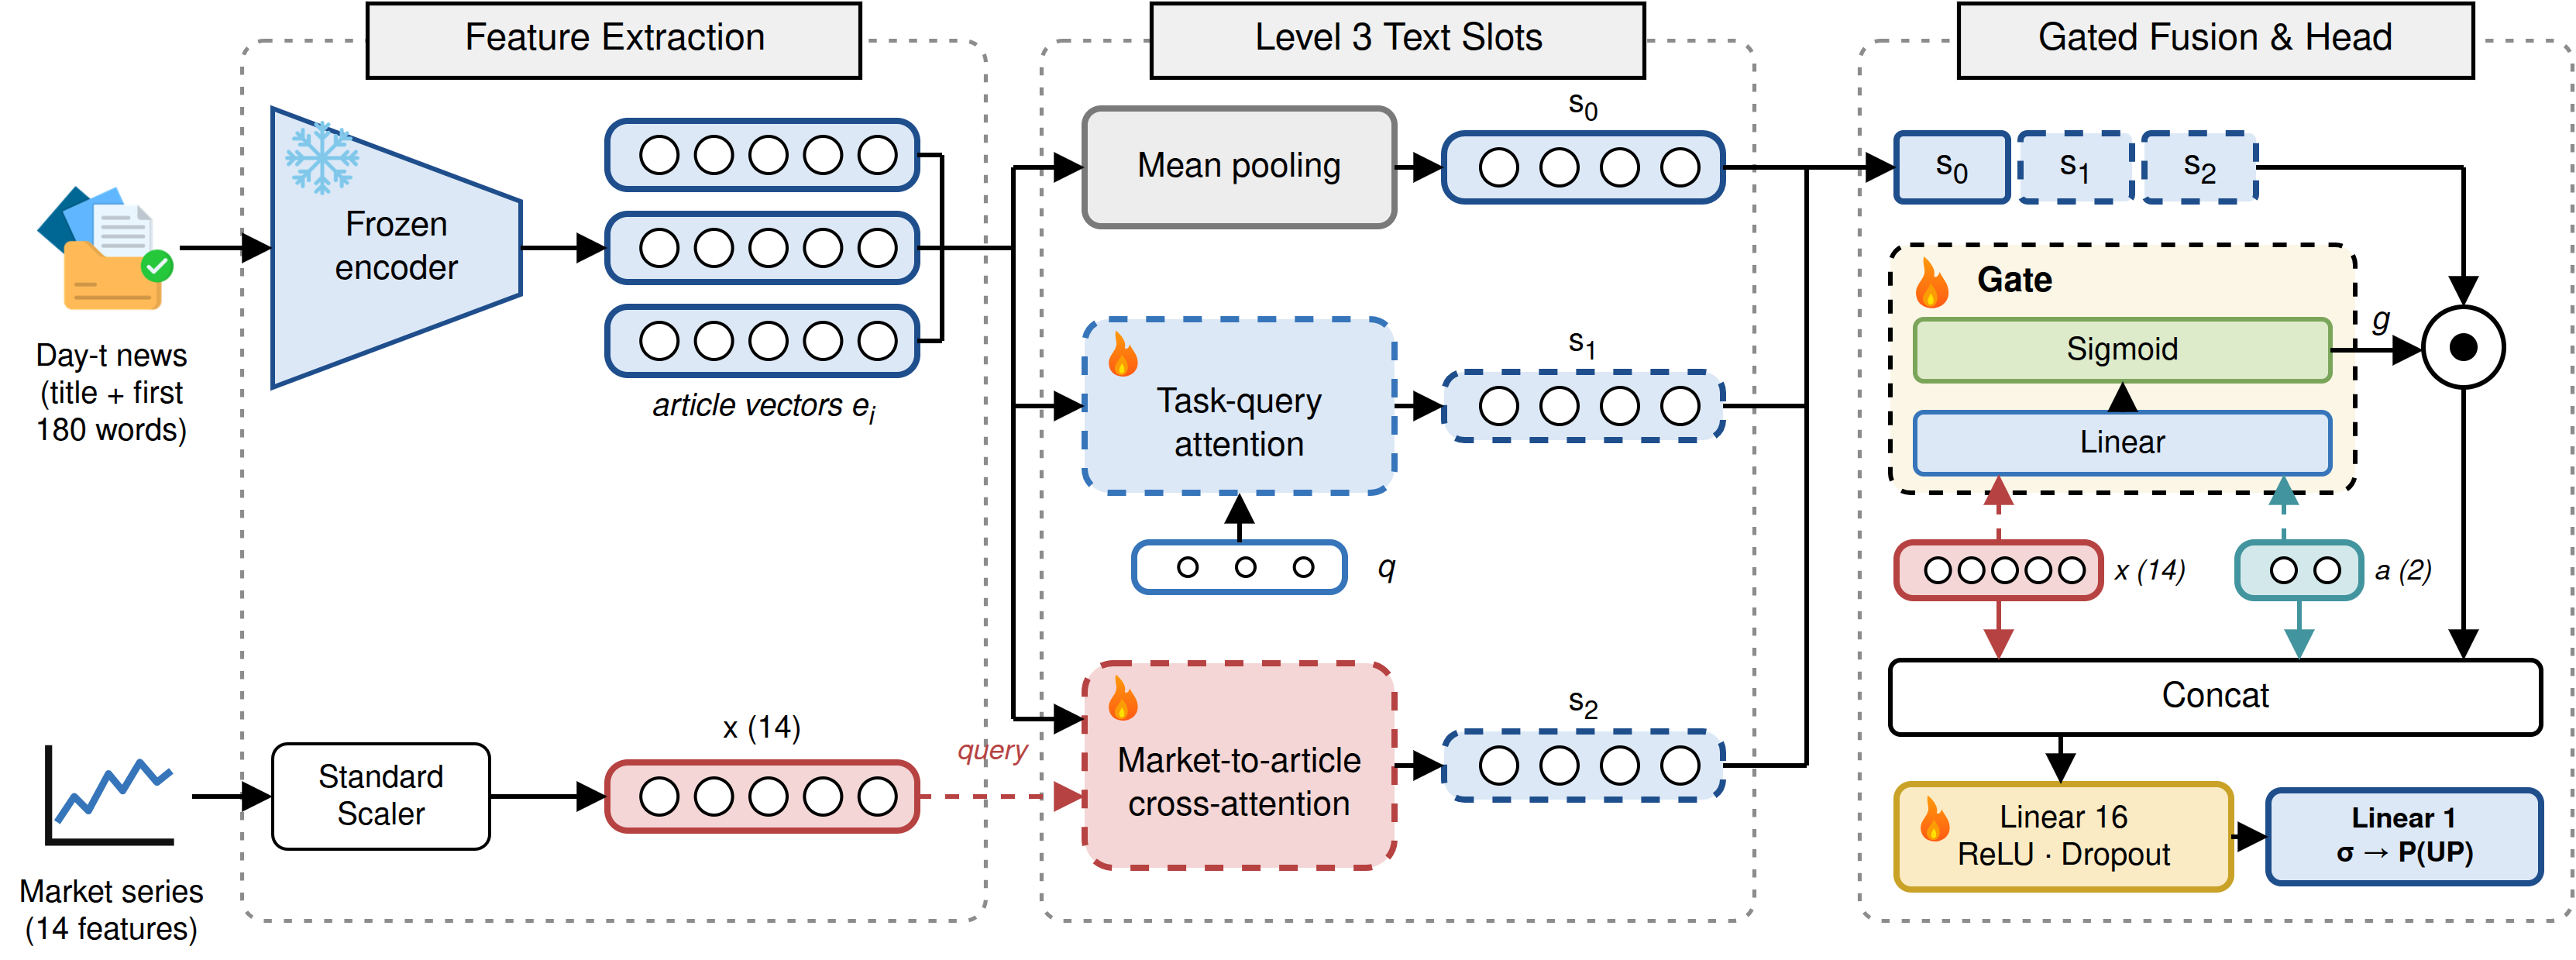
\includegraphics[width=\textwidth]{model_architecture.png}
    \caption{Level~3 architecture. A frozen encoder gives a 768-dimensional vector $\mathbf{e}_i$ per article. The mean slot $\mathbf{s}_0$ is always on. Dashed components switch on in addition to it: the task-query slot $\mathbf{s}_1$, the cross-attention slot $\mathbf{s}_2$, and the scalar gate. Slots are concatenated, and inactive slots are zero vectors. The gate reads the 14 market inputs $\mathbf{x}$ and the log article count, the first availability input, and $\odot$ scales all slots by the gate value $g$. $\mathbf{x}$ and both availability inputs $\mathbf{a}$ also join the concatenation. Flames mark trained parts and the snowflake marks the frozen encoder.}
    \label{fig:architecture}
\end{figure*}

